\subsection{Задание 2}%
\label{subsec:2}%
Исходные данные неупорядоченные:\newline%
\newline%
%
\begin{changemargin}{-4cm}{0cm}\small{%
\begin{tabular}{|p{0.08\linewidth}|p{0.08\linewidth}|p{0.08\linewidth}|p{0.08\linewidth}|p{0.08\linewidth}|p{0.08\linewidth}|p{0.08\linewidth}|p{0.08\linewidth}|p{0.08\linewidth}|p{0.08\linewidth}|}%
\hline%
9.77025&7.84276&4.05229&8.04839&9.41659&7.57213&8.61462&4.95985&5.77880&3.12317\\%
\hline%
6.49458&6.94320&7.57100&5.36951&10.55283&7.51243&9.63317&7.53753&8.82055&6.50139\\%
\hline%
6.49341&7.28528&7.70446&5.49125&7.63095&5.17903&6.71337&6.80843&5.16512&7.49481\\%
\hline%
9.30528&11.52394&3.91187&3.55400&4.16010&7.72491&6.91488&7.51121&8.76289&7.19596\\%
\hline%
8.78022&2.82677&7.01889&5.42802&7.18210&9.69690&4.96187&7.61321&5.05334&6.95743\\%
\hline%
6.33703&8.43742&7.40592&8.14157&5.76268&5.62357&5.76960&5.52992&5.71038&6.96062\\%
\hline%
8.28251&8.01207&5.86276&6.09561&5.62196&7.47430&5.87784&3.23621&5.41288&7.68933\\%
\hline%
4.20785&7.28157&8.33969&6.13279&8.24552&8.80064&6.69964&8.66011&10.73090&7.39790\\%
\hline%
7.59231&5.37157&4.72374&9.13526&1.96161&6.31527&8.98943&6.05701&7.56973&6.31533\\%
\hline%
5.11918&8.28191&7.52606&5.52857&5.88576&6.16393&5.44642&4.29147&8.30444&6.62887\\%
\hline%
6.47003&7.02147&7.61848&6.99433&6.89876&6.14050&7.73999&6.04531&8.87165&6.89893\\%
\hline%
8.27708&6.89119&4.35793&7.42013&6.58775&8.27541&6.87410&8.53980&8.56065&8.22202\\%
\hline%
6.22377&6.89487&7.74233&8.80423&9.33313&6.57722&5.06884&8.40925&8.12839&7.98477\\%
\hline%
8.26201&4.93473&5.12688&4.41217&9.51142&6.40781&7.50593&5.35190&5.74046&6.14165\\%
\hline%
4.97357&9.22183&6.04206&4.40426&9.51716&5.25917&6.73307&7.01934&7.13955&6.28469\\%
\hline%
8.26906&8.16409&4.80252&6.95316&6.76033&5.75203&7.32998&6.77154&6.79967&4.34950\\%
\hline%
6.22581&9.33770&7.04449&5.20514&9.45650&5.22006&5.42706&5.96046&6.29732&9.65425\\%
\hline%
4.20325&7.23606&4.52708&5.60927&6.47370&3.43781&6.61158&7.68103&6.63923&8.43593\\%
\hline%
7.74532&7.13404&7.65328&7.21342&7.00606&8.11294&5.81466&5.60671&9.30283&11.38605\\%
\hline%
9.06896&5.46313&9.29720&6.04036&8.29306&7.72403&6.48576&6.43837&7.49219&4.69380\\%
\hline%
\end{tabular}%
\newline%
\newline%
%
}\end{changemargin}%
\newpage%
Исходные данные упорядоченные:\newline%
\newline%
%
\begin{changemargin}{-4cm}{0cm}\small{%
\begin{tabular}{|p{0.08\linewidth}|p{0.08\linewidth}|p{0.08\linewidth}|p{0.08\linewidth}|p{0.08\linewidth}|p{0.08\linewidth}|p{0.08\linewidth}|p{0.08\linewidth}|p{0.08\linewidth}|p{0.08\linewidth}|}%
\hline%
1.96161&2.82677&3.12317&3.23621&3.43781&3.55400&3.91187&4.05229&4.16010&4.20325\\%
\hline%
4.20785&4.29147&4.34950&4.35793&4.40426&4.41217&4.52708&4.69380&4.72374&4.80252\\%
\hline%
4.93473&4.95985&4.96187&4.97357&5.05334&5.06884&5.11918&5.12688&5.16512&5.17903\\%
\hline%
5.20514&5.22006&5.25917&5.35190&5.36951&5.37157&5.41288&5.42706&5.42802&5.44642\\%
\hline%
5.46313&5.49125&5.52857&5.52992&5.60671&5.60927&5.62196&5.62357&5.71038&5.74046\\%
\hline%
5.75203&5.76268&5.76960&5.77880&5.81466&5.86276&5.87784&5.88576&5.96046&6.04036\\%
\hline%
6.04206&6.04531&6.05701&6.09561&6.13279&6.14050&6.14165&6.16393&6.22377&6.22581\\%
\hline%
6.28469&6.29732&6.31527&6.31533&6.33703&6.40781&6.43837&6.47003&6.47370&6.48576\\%
\hline%
6.49341&6.49458&6.50139&6.57722&6.58775&6.61158&6.62887&6.63923&6.69964&6.71337\\%
\hline%
6.73307&6.76033&6.77154&6.79967&6.80843&6.87410&6.89119&6.89487&6.89876&6.89893\\%
\hline%
6.91488&6.94320&6.95316&6.95743&6.96062&6.99433&7.00606&7.01889&7.01934&7.02147\\%
\hline%
7.04449&7.13404&7.13955&7.18210&7.19596&7.21342&7.23606&7.28157&7.28528&7.32998\\%
\hline%
7.39790&7.40592&7.42013&7.47430&7.49219&7.49481&7.50593&7.51121&7.51243&7.52606\\%
\hline%
7.53753&7.56973&7.57100&7.57213&7.59231&7.61321&7.61848&7.63095&7.65328&7.68103\\%
\hline%
7.68933&7.70446&7.72403&7.72491&7.73999&7.74233&7.74532&7.84276&7.98477&8.01207\\%
\hline%
8.04839&8.11294&8.12839&8.14157&8.16409&8.22202&8.24552&8.26201&8.26906&8.27541\\%
\hline%
8.27708&8.28191&8.28251&8.29306&8.30444&8.33969&8.40925&8.43593&8.43742&8.53980\\%
\hline%
8.56065&8.61462&8.66011&8.76289&8.78022&8.80064&8.80423&8.82055&8.87165&8.98943\\%
\hline%
9.06896&9.13526&9.22183&9.29720&9.30283&9.30528&9.33313&9.33770&9.41659&9.45650\\%
\hline%
9.51142&9.51716&9.63317&9.65425&9.69690&9.77025&10.55283&10.73090&11.38605&11.52394\\%
\hline%
\end{tabular}%
\newline%
\newline%
%
}\end{changemargin}%
\newpage%
Группированная выборка:\newline%
\newline%
%
\begin{tabular}{|c|c|c|}%
\hline%
Интервалы&$n_i$&$w_i$\\%
\hline%
{[}1.96161,3.15690{]}&3.00000&0.01500\\%
\hline%
{[}3.15690,4.35219{]}&10.00000&0.05000\\%
\hline%
{[}4.35219,5.54748{]}&31.00000&0.15500\\%
\hline%
{[}5.54748,6.74277{]}&47.00000&0.23500\\%
\hline%
{[}6.74277,7.93807{]}&57.00000&0.28500\\%
\hline%
{[}7.93807,9.13336{]}&33.00000&0.16500\\%
\hline%
{[}9.13336,10.32865{]}&15.00000&0.07500\\%
\hline%
{[}10.32865,11.52394{]}&4.00000&0.02000\\%
\hline%
{-}&200.00000&1.00000\\%
\hline%
\end{tabular}%
\newline%
\newline%
%
Построим оценки математического ожидания и дисперсии:\newline%
\newline%
%
$\widetilde{a} = \overline{\mu_1}=$6.88621$;\widetilde{\sigma}^2 =$2.92259%
\newpage%
\begin{tabular}{|c|c|c|c|c|c|}%
\hline%
$k$&$a_k$&$\frac{a_k - \widetilde{a}}{\sigma}$&$\frac{1}{\sigma} \varphi( \frac{a_k - \widetilde{a}}{\sigma} )$&$ \Phi( \frac{a_k - \widetilde{a}}{\sigma} )$&$p_{k}^*$\\%
\hline%
0.00000&1.96161&{-}2.88063&0.00368&0.00198&{-}\\%
\hline%
1.00000&3.15690&{-}2.18144&0.02161&0.01458&0.01458\\%
\hline%
2.00000&4.35219&{-}1.48226&0.07779&0.06914&0.05456\\%
\hline%
3.00000&5.54748&{-}0.78308&0.17174&0.21679&0.14765\\%
\hline%
4.00000&6.74277&{-}0.08390&0.23254&0.46657&0.24978\\%
\hline%
5.00000&7.93807&0.61528&0.19312&0.73081&0.26425\\%
\hline%
6.00000&9.13336&1.31446&0.09836&0.90565&0.17484\\%
\hline%
7.00000&10.32865&2.01364&0.03073&0.97798&0.07232\\%
\hline%
8.00000&11.52394&2.71282&0.00589&0.99666&0.02202\\%
\hline%
{-}&{-}&{-}&{-}&{-}&$\sum p_{k}^*=$1.00000\\%
\hline%
\end{tabular}%
\newline%
\newline%
%
\begin{changemargin}{-4cm}{0cm}\small{%
\begin{tabular}{|c|c|c|c|c|c|}%
\hline%
$k$&Интервал&$w_k$&$p_{k}^*$&$|w_i-p_{i}^*|$&$\frac{N(w_k - p_k)^2}{p_{k}^*}$\\%
\hline%
1.00000&{[}1.96161, 3.15690{]}&0.01500&0.01458&0.00042&0.00248\\%
\hline%
2.00000&{[}3.15690, 4.35219{]}&0.05000&0.05456&0.00456&0.07622\\%
\hline%
3.00000&{[}4.35219, 5.54748{]}&0.15500&0.14765&0.00735&0.07309\\%
\hline%
4.00000&{[}5.54748, 6.74277{]}&0.23500&0.24978&0.01478&0.17487\\%
\hline%
5.00000&{[}6.74277, 7.93807{]}&0.28500&0.26425&0.02075&0.32595\\%
\hline%
6.00000&{[}7.93807, 9.13336{]}&0.16500&0.17484&0.00984&0.11075\\%
\hline%
7.00000&{[}9.13336, 10.32865{]}&0.07500&0.07232&0.00268&0.01983\\%
\hline%
8.00000&{[}10.32865, 11.52394{]}&0.02000&0.02202&0.00202&0.03719\\%
\hline%
{-}&{-}&$\sum w_k=$1.00000&$\sum p_{k}^*=$1.00000&$max | w_i - p_{i}^*|=$0.02075&$\frac{N(w_k - p_k)^2}{p_{k}^*}$=0.82037\\%
\hline%
\end{tabular}%
\newline%
\newline%
%
}\end{changemargin}%
\newpage%


\begin{figure}%
\centering%
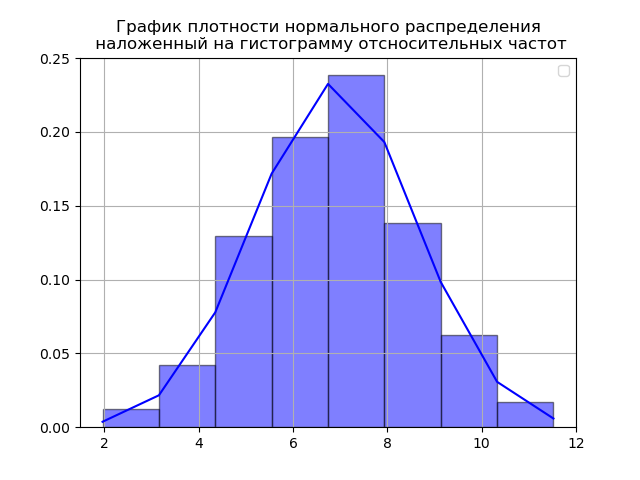
\includegraphics[width=1.0\textwidth]{../latex/inc/generated/img/relFreqDensity3.png}%
\end{figure}

%
$m=8 \quad l=m-3=5$

%
$\chi_{B}^2 = 0.82037 \quad \chi^2_{\text{кр}, \alpha}(5) = 11.10000$

%
$0.82037 \le 11.1$%
, то гипотеза о соответствии выборки нормальному распределению не противоречит экспериментальным данным при уровне значимости $a=0,05$